\section{Introduction} \label{man-introduction}
This section will go in detail about the workings, idea's and logic of our
database and queries.

\section{Application} \label{man-application}
The database is based the expert system we have built in the previous
assignment. This system identifies the vehicle type based on user input.

By answering specific questions that the expert system asks,
the system is able to deduce and identify the type of a vehicle.
An example of a vehicle type defined in our system is `land vehicle'.
A land vehicle, like other vehicle types in our system, also consists
of subtypes. Subtypes of land vehicles are cars and bicycles in our expert system.

By answering `yes' or `no' to certain questions,
the expert system is able to make an educated
guess about the type of the vehicle.

This database and accompanying queries tries to translate this functionality
into a database. Some vehicle data is inserted into tables. Vehicle subtypes
each have their on table in our database (air vehicle, land vehicle,
water vehicle). These three tables are merged into a bigger and more general
`vehicles' table. This `vehicles' table is queried simulating the our vehicle
types expert system.

\subsection{Flowchart} \label{man-diagram-application}
\begin{figure}[H]
  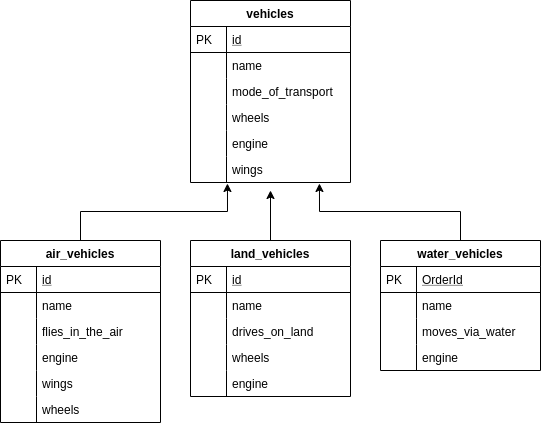
\includegraphics[width=\linewidth]{images/VehicleTypesRTables.png}
  \caption{This figure shows a visual representation of our vehicle types database schema}
\end{figure}

\section{Usage} \label{man-usage}
The application is run by providing the following command \textbf{Rscript pa2.r}
(Remove the `.txt' extension from the file if you haven't done so already).

Runnin initializes all functions, tables, queries and other data needed for the
program. It also executes all queries at once along with a helpful message
telling the user what the query has tried to retrieve from the database.

\newpage
\section{Queries} \label{man-queries}
Below will be listed several queries that each test a rule in our expert system.
The queries will be listed along with the responses of the system and comments
providing extra information.

\begin{lstlisting}{}
Query: vehicles <- full_join(air_vehicles, land_vehicles) %>% full_join(water_vehicles) %>% replace(is.na(.),FALSE)

Result:
% Showing all vehicles in a table
% # A tibble: 9 x 8
     % id name  flies\_in\_the\_air engine wings wheels drives\_on\_land
  % <dbl> <chr> <lgl>            <lgl>  <lgl>  <dbl> <lgl>
     % 1 Airb... TRUE             TRUE   TRUE      20 FALSE
     % 2 Apol... TRUE             TRUE   FALSE      0 FALSE
     % 3 Lock... TRUE             TRUE   TRUE       6 FALSE
     % 1 Ferr... FALSE            TRUE   FALSE      4 TRUE
     % 2 Gaze... FALSE            FALSE  FALSE      2 TRUE
     % 3 Yama... FALSE            TRUE   FALSE      2 TRUE
     % 1 Rega... FALSE            TRUE   FALSE      0 FALSE
     % 2 Lizz... FALSE            FALSE  FALSE      0 FALSE
     % 3 Lazz... FALSE            TRUE   FALSE      0 FALSE
% # ... with 1 more variable: moves\_via\_water <lgl>
\end{lstlisting}

\begin{lstlisting}{}
Query:
bicycles <- vehicles %>% filter(drives_on_land == TRUE, wheels == 2, engine == FALSE)

Result:
% Showing all bicycles in a table
% # A tibble: 1 x 8
     % id name  flies\_in\_the\_air engine wings wheels drives\_on\_land
  % <dbl> <chr> <lgl>            <lgl>  <lgl>  <dbl> <lgl>
% 1     2 Gaze... FALSE            FALSE  FALSE      2 TRUE
% # ... with 1 more variable: moves\_via\_water <lgl>
\end{lstlisting}

\begin{lstlisting}{}
Query:
motor_bikes <- vehicles %>% filter(drives_on_land == TRUE, wheels == 2, engine == TRUE)

Result:
% Showing all motor bikes in a table
%
% # A tibble: 1 x 8
     % id name  flies_in_the_air engine wings wheels drives_on_land
  % <dbl> <chr> <lgl>            <lgl>  <lgl>  <dbl> <lgl>
% 1     3 Yama... FALSE            TRUE   FALSE      2 TRUE
% # ... with 1 more variable: moves_via_water <lgl>
\end{lstlisting}

\begin{lstlisting}{}
Query:
cars <- vehicles %>% filter(drives_on_land == TRUE, wheels == 4, engine == FALSE)

Result:
% Showing all cars in a table
%
% # A tibble: 0 x 8
% # ... with 8 variables: id <dbl>, name <chr>, flies_in_the_air <lgl>,
% #   engine <lgl>, wings <lgl>, wheels <dbl>, drives_on_land <lgl>,
% #   moves_via_water <lgl>
\end{lstlisting}

\begin{lstlisting}{}
Query:
airplanes <- vehicles %>% filter(flies_in_the_air == TRUE, wings == TRUE, engine == TRUE, wheels > 3)

Result:
% Showing all airplanes in a table
%
% # A tibble: 2 x 8
     % id name  flies_in_the_air engine wings wheels drives_on_land
  % <dbl> <chr> <lgl>            <lgl>  <lgl>  <dbl> <lgl>
% 1     1 Airb... TRUE             TRUE   TRUE      20 FALSE
% 2     3 Lock... TRUE             TRUE   TRUE       6 FALSE
% # .... with 1 more variable: moves_via_water <lgl>
\end{lstlisting}

\begin{lstlisting}{}
Query:
space_crafts <- vehicles %>% filter(flies_in_the_air == TRUE, engine == TRUE, wheels == 0)


Result:
% Showing all space crafts in a table
%
% # A tibble: 1 x 8
     % id name  flies_in_the_air engine wings wheels drives_on_land
  % <dbl> <chr> <lgl>            <lgl>  <lgl>  <dbl> <lgl>
% 1     2 Apol... TRUE             TRUE   FALSE      0 FALSE
% # ... with 1 more variable: moves_via_water <lgl>
\end{lstlisting}

\begin{lstlisting}{}
Query:
boats <- vehicles %>% filter(moves_via_water == TRUE)

Result:
% Showing all boats in a table
%
% # A tibble: 3 x 8
     % id name  flies\_in\_the\_air engine wings wheels drives_on_land
  % <dbl> <chr> <lgl>            <lgl>  <lgl>  <dbl> <lgl>
% 1     1 Rega... FALSE            TRUE   FALSE      0 FALSE
% 2     2 Lizz... FALSE            FALSE  FALSE      0 FALSE
% 3     3 Lazz... FALSE            TRUE   FALSE      0 FALSE
% # ... with 1 more variable: moves_via_water <lgl>
\end{lstlisting}

\newpage

\section{Logical Correspondence between current program and expert system}
\begin{table}[H]
\centering
\resizebox{\textwidth}{!}{%
\begin{tabular}{ll} \hline
  \multicolumn{1}{|l|}{\textbf{Database}} & \multicolumn{1}{l|}{\textbf{Logical Correspondence}}\\ \hline
  \multicolumn{1}{|l|}{vehicles \textless- full\_join(air\_vehicles, land\_vehicles)
    \%\textgreater{}\% full\_join(water\_vehicles)...} &
    \multicolumn{1}{|l|}{$A \cup L \cup W   =   \{t | t \in A \bigvee t \in L
    \bigvee t \in W\}$} \\ \hline
  \multicolumn{1}{|l|}{bicycles \textless- vehicles \%\textgreater\%
  filter(drives\_on\_land == TRUE, wheels == 2, engine == FALSE)} &
    \multicolumn{1}{|l|}{$\{t | t \in LandVehicles \bigwedge t.wheels = 2
    \bigwedge t.engine = false)\}$} \\ \hline
  \multicolumn{1}{|l|}{motor\_bikes \textless- vehicles \%\textgreater\%
  filter(drives\_on\_land == TRUE, wheels == 2, engine == TRUE)} &
    \multicolumn{1}{|l|}{$\{t | t \in LandVehicles \bigwedge t.wheels = 2
    \bigwedge t.engine = true)\}$} \\ \hline
  \multicolumn{1}{|l|}{cars \textless- vehicles \%\textgreater\%
  filter(drives\_on\_land == TRUE, wheels == 4, engine == TRUE)} &
    \multicolumn{1}{|l|}{$\{t | t \in LandVehicles \bigwedge t.wheels = 4
    \bigwedge t.engine = true)\}$} \\ \hline
  \multicolumn{1}{|l|}{airplanes \textless- vehicles \%\textgreater\%
  filter(flies\_in\_the\_air == TRUE, wings == TRUE, engine == TRUE, wheels > 3)} &
    \multicolumn{1}{|l|}{$\{t | t \in AirVehicles \bigwedge t.wings = true
    \bigwedge t.engine = true \bigwedge t.wheels > 3)\}$} \\ \hline
  \multicolumn{1}{|l|}{space\_crafts \textless- vehicles \%\textgreater\%
  filter(flies\_in\_the\_air == TRUE, engine == TRUE, wheels == 0)} &
    \multicolumn{1}{|l|}{$\{t | t \in AirVehicles \bigwedge t.wheels = 0
    \bigwedge t.engine = true)\}$} \\ \hline
  \multicolumn{1}{|l|}{boats \textless- vehicles \%\textgreater\%
  filter(moves\_on\_water == TRUE)} &
    \multicolumn{1}{|l|}{$\{t | t \in WaterVehicles\}$} \\ \hline
\end{tabular}%
}
\end{table}
